\documentclass[12pt,a4paper]{article}

\usepackage[a4paper,margin=2.2cm]{geometry}
\usepackage[T2A]{fontenc}
\usepackage[utf8]{inputenc}
\usepackage[russian]{babel}
\usepackage{amsmath,amssymb,mathtools}
\usepackage{graphicx}
\usepackage{float}
\usepackage{hyperref}
\hypersetup{colorlinks=true,linkcolor=black,urlcolor=blue}

\title{Assignment 3\\EM-алгоритм для детектива}
\author{}
\date{}

\begin{document}
\maketitle

\section*{Что сделано}

В работе реализованы все основные части задания:
\begin{itemize}
    \item теоретически выведены формулы для E-шагa, M-шагa и нижней оценки;
    \item реализованы обычный EM и hard EM в файле \texttt{Student.py};
    \item добавлен многократный запуск из разных инициализаций \texttt{run\_EM\_with\_restarts};
    \item добавлена генерация маленьких синтетических данных;
    \item эксперименты вынесены в файл \texttt{run\_experiments.py};
    \item открытые тесты вынесены в удобный запуск \texttt{run\_tests.py};
    \item добавлена регрессионная проверка, что матрица $A$ остаётся нормированным распределением даже при повторяющихся MAP-сдвигах;
    \item собраны примеры результатов на синтетических и реальных данных.
\end{itemize}

\section{Модель}

Есть выборка изображений $X = \{X_k\}_{k=1}^{K}$ размера $H \times W$. На каждом изображении:
\begin{itemize}
    \item общий фон $B \in \mathbb{R}^{H \times W}$;
    \item лицо $F \in \mathbb{R}^{h \times w}$;
    \item скрытый сдвиг $d_k = (d_k^h, d_k^w)$;
    \item независимый гауссов шум $\mathcal{N}(0, s^2)$.
\end{itemize}

Если пиксель попадает в прямоугольник лица, его среднее равно соответствующему пикселю из $F$, иначе --- пикселю из $B$. Априорное распределение на координаты задаётся матрицей $A$:
\[
p(d_k = (i,j) \mid A) = A(i,j),
\qquad
\sum_{ij} A(i,j) = 1.
\]

Совместная модель имеет вид
\[
p(X,d \mid \theta, A) = \prod_{k=1}^{K} p(X_k \mid d_k,\theta)\, p(d_k \mid A),
\qquad
\theta = \{F,B,s^2\}.
\]

\section{Теория}

\subsection*{1. E-шаг}

Для каждого изображения и каждого допустимого сдвига:
\[
p(d_k \mid X_k,\theta,A) \propto p(X_k \mid d_k,\theta)\, A(d_k).
\]

В логарифмах это записывается так:
\[
\log q_k(d) = \log p(X_k \mid d,\theta) + \log A(d) - C_k,
\]
где $C_k$ --- нормировочная константа. При вычислении $q_k$ используется устойчивая нормировка:
\[
\frac{e^{\alpha_i}}{\sum_j e^{\alpha_j}}
=
\frac{e^{\alpha_i - \max_j \alpha_j}}{\sum_j e^{\alpha_j - \max_j \alpha_j}},
\]
что избавляет от переполнения и потери точности.

В hard EM вместо полного распределения берётся только MAP-оценка
\[
d_k^{MAP} = \arg\max_d p(d \mid X_k,\theta,A).
\]

\subsection*{2. M-шаг}

Параметры пересчитываются именно в порядке $A, F, B, s^2$.

\paragraph{Оценка $A$.}
\[
A(d) = \frac{1}{K}\sum_{k=1}^{K} q_k(d).
\]
В hard EM это просто частоты MAP-сдвигов.

\paragraph{Оценка лица $F$.}
\[
F(u,v) = \frac{1}{K} \sum_{k=1}^{K} \sum_d q_k(d)\, X_k(d^h + u, d^w + v).
\]
То есть каждый пиксель лица --- это взвешенное среднее по всем изображениям и всем возможным положениям лица.

\paragraph{Оценка фона $B$.}
Пусть
\[
r_{ijk} = 1 - \sum_d q_k(d)\, \mathbf{1}\{(i,j)\in faceArea(d)\}
\]
--- вероятность того, что пиксель $(i,j)$ на изображении $k$ относится к фону. Тогда
\[
B(i,j) = \frac{\sum_k r_{ijk}X_k(i,j)}{\sum_k r_{ijk}}.
\]

\paragraph{Оценка шума $s^2$.}
\[
s^2 = \frac{1}{KHW} \sum_{k=1}^{K}\sum_d q_k(d)\sum_{i,j}
\Bigl(X_k(i,j) - \mu_{ij}(d)\Bigr)^2,
\]
где $\mu_{ij}(d)$ равно либо пикселю из $F$, либо пикселю из $B$, в зависимости от того, попадает ли $(i,j)$ в область лица.

\subsection*{3. Нижняя оценка}

Оптимизируется стандартная нижняя оценка EM:
\[
\mathcal{L}(q,\theta,A) =
\sum_k \sum_d q_k(d)
\Bigl(\log p(X_k \mid d,\theta) + \log A(d) - \log q_k(d)\Bigr).
\]

Для hard EM энтропийный член исчезает, потому что $q_k(d)$ вырождено: в одной точке оно равно $1$, а в остальных равно $0$.

\section{Реализация}

\subsection*{Пункт 1. Полный EM-алгоритм}

Реализованы все требуемые функции:
\begin{itemize}
    \item \texttt{calculate\_log\_probability} считает $\log p(X_k \mid d_k,\theta)$ для всех сдвигов;
    \item \texttt{run\_e\_step} вычисляет постериорное распределение по координатам;
    \item \texttt{run\_m\_step} пересчитывает $A, F, B, s$;
    \item \texttt{calculate\_lower\_bound} считает $\mathcal{L}(q,\theta,A)$;
    \item \texttt{run\_EM} выполняет цикл E-шаг $\rightarrow$ M-шаг $\rightarrow$ вычисление нижней оценки.
\end{itemize}

Критерий остановки exactly соответствует постановке:
\[
\mathcal{L}_{t+1} - \mathcal{L}_t < tol.
\]
В реализации на каждой итерации сначала фиксируется $q$ после E-шагa, затем считается прирост
\[
\mathcal{L}(q,\theta^{(t+1)},A^{(t+1)}) -
\mathcal{L}(q,\theta^{(t)},A^{(t)}),
\]
то есть сравниваются параметры до и после M-шагa при одном и том же распределении $q$.

\subsection*{Пункт 2. Hard EM}

Для hard EM добавлен режим \texttt{use\_MAP=True}. В этом случае после E-шагa остаётся не всё распределение по сдвигам, а только один лучший сдвиг для каждого изображения.
При подсчёте $A$ частоты MAP-сдвигов аккумулируются с учётом повторяющихся координат, поэтому $\sum_d A(d)=1$ сохраняется и в hard EM, и в случае вырожденного soft posterior.

\subsection*{Пункт 3. Несколько запусков}

Это сделано в \texttt{run\_EM\_with\_restarts}. Функция запускает EM несколько раз и берёт тот результат, у которого нижняя оценка в конце больше.

\subsection*{Пункт 4. Синтетические данные}

В \texttt{run\_experiments.py} есть функция \texttt{generate\_toy\_data}. Она строит маленькие изображения $20 \times 30$ с одним и тем же фоном, объектом $15 \times 15$ и нормальным шумом. Эти данные нужны для быстрой отладки и простых сравнений.

\section{Результаты и анализ}

\subsection*{Примеры восстановлений}

Для синтетических данных сохраняется \texttt{results/toy\_reconstruction.png}, а для данных из задания --- \texttt{results/real\_reconstruction.png}. На этих картинках показаны оценки лица $F$ и фона $B$.

\begin{figure}[H]
\centering
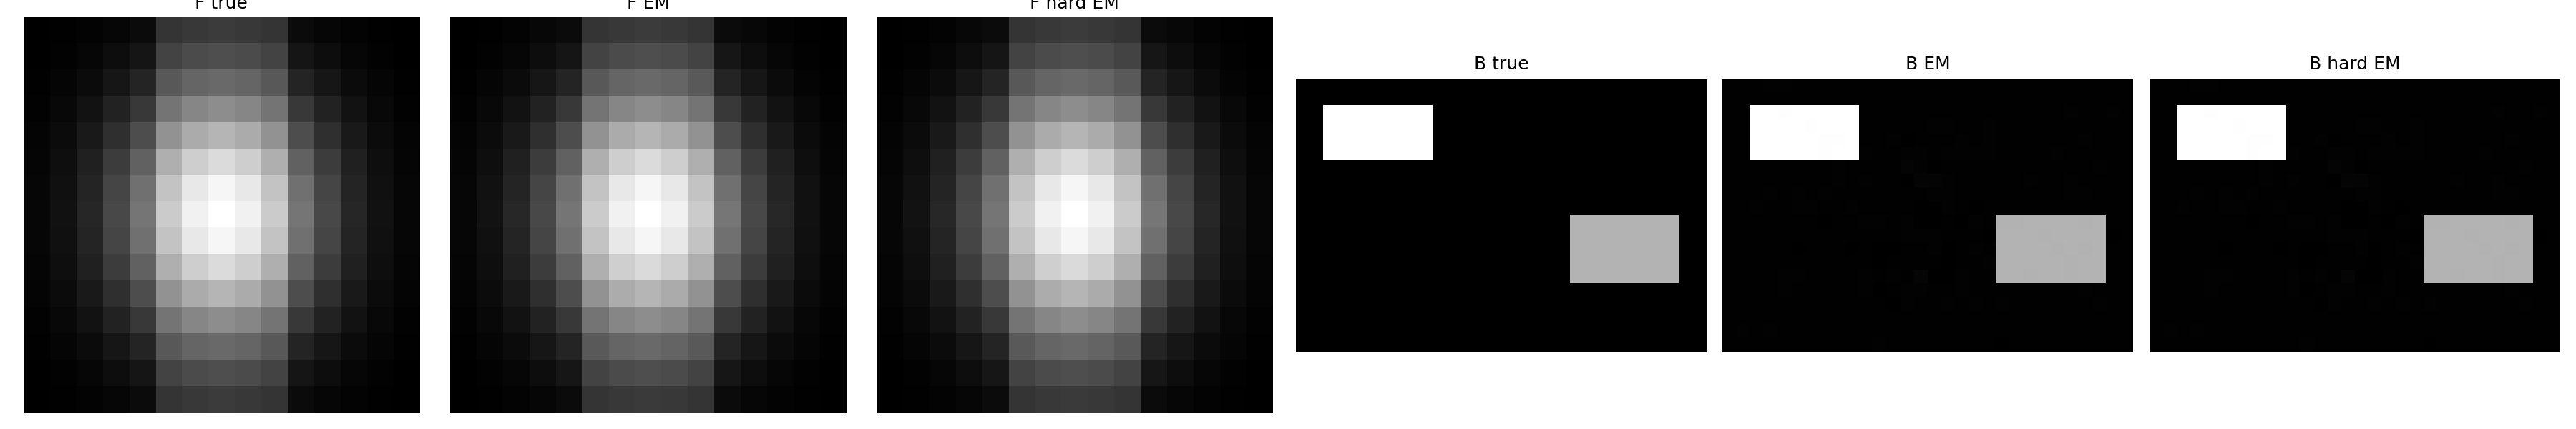
\includegraphics[width=0.95\textwidth]{results/toy_reconstruction.png}
\caption{Пример восстановления лица и фона на синтетических данных.}
\end{figure}

\begin{figure}[H]
\centering
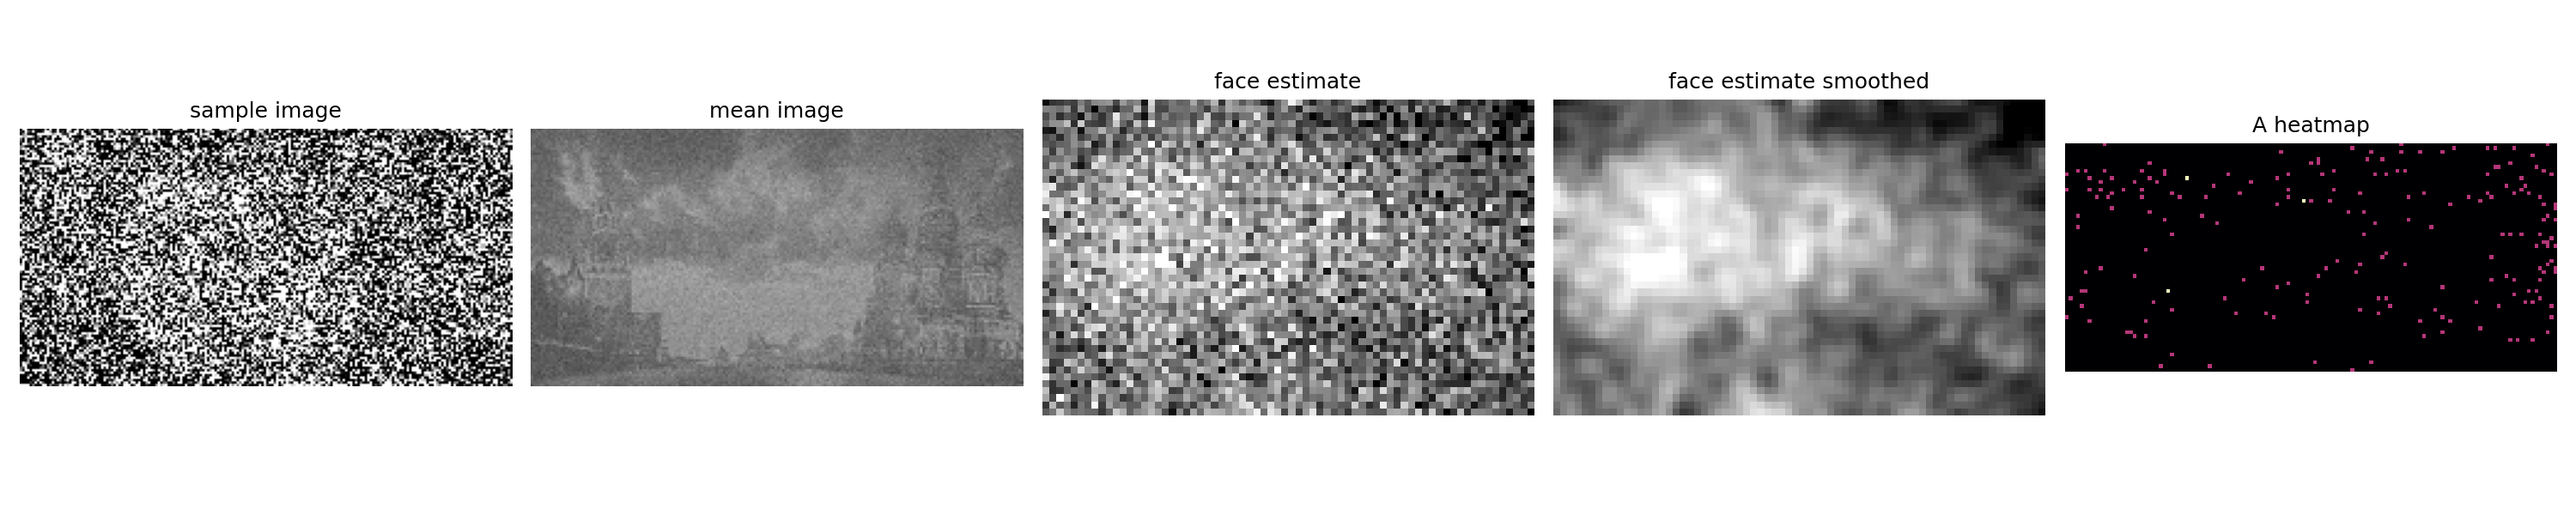
\includegraphics[width=0.95\textwidth]{results/real_reconstruction.png}
\caption{Визуализация на реальных данных: образец кадра, среднее по 200 кадрам, контрастно нормированная оценка лица, её сглаженная версия и тепловая карта $A$.}
\end{figure}

\subsection*{1. Влияние начального приближения}

На синтетической выборке с $K=20$ и шумом $0.6$ были сделаны 4 запуска с разными seed. Результаты заметно различались:
\begin{itemize}
    \item лучший запуск: $\mathcal{L} \approx -49782.65$, $\mathrm{MSE}(F) \approx 2425.42$, $\mathrm{MSE}(B) \approx 96.08$;
    \item худший запуск: $\mathcal{L} \approx -56056.47$, $\mathrm{MSE}(F) \approx 8711.84$, $\mathrm{MSE}(B) \approx 907.55$.
\end{itemize}

Значит, начальное приближение влияет сильно. Из-за локальных максимумов один запуск EM здесь ненадёжен, поэтому рестарты полезны.

\subsection*{2. Влияние размера выборки и шума}

На синтетических данных были сделаны короткие прогоны при разных $K$ и уровнях шума. Для сравнения использовалось нормированное значение $\mathcal{L}/(KHW)$.

\paragraph{Размер выборки.}
\begin{itemize}
    \item $K=10$: $\mathcal{L}/(KHW) \approx -4.156$, $\mathrm{MSE}(F) \approx 2247.29$;
    \item $K=20$: $\mathcal{L}/(KHW) \approx -4.669$, $\mathrm{MSE}(F) \approx 9195.76$;
    \item $K=30$: $\mathcal{L}/(KHW) \approx -3.984$, $\mathrm{MSE}(F) \approx 2597.94$.
\end{itemize}

\paragraph{Шум.}
При увеличении шума качество ожидаемо падает: лицо и фон восстанавливаются хуже, а оценка $\sigma$ растёт.

\subsection*{3. Сравнение EM и hard EM}

На одной и той же синтетической выборке получилось:
\begin{itemize}
    \item EM: время $\approx 0.175$ сек, $\mathcal{L}/(KHW) \approx -3.713005$;
    \item hard EM: время $\approx 0.073$ сек, $\mathcal{L}/(KHW) \approx -3.713236$.
\end{itemize}

На этом примере hard EM оказался примерно в $2.4$ раза быстрее. Качество почти совпало, но обычный EM в целом надёжнее, потому что использует всё распределение по сдвигам, а не только один максимум.

После исправления нормировки $A$ основной прогон из \texttt{run\_experiments.py} даёт одинаковую оценку шума для EM и hard EM, $\sigma \approx 0.587$, а итоговая нижняя оценка на синтетической выборке стала
\[
\mathcal{L} \approx -21411.89.
\]

\subsection*{4. Реальные данные}

На реальных данных выяснилось, что проблема была не только в тяжёлом шуме, но и в визуализации: если рисовать оценку лица в диапазоне $[0,255]$, слабая структура почти полностью теряется и панель выглядит как серый шум. Поэтому для итоговой картинки оценка лица показывается с отдельной контрастной нормировкой по квантилям, а матрица $A$ рисуется как тепловая карта, а не как обычное серое изображение.

Кроме того, для preview лица использовалась более устойчивая инициализация по 200 кадрам.
Численный EM-контроль считался на короткой подвыборке; его итог:
\[
\mathcal{L} \approx -1019025.62,
\qquad
\sigma \approx 104.23.
\]

На реальных данных задача заметно тяжелее, чем на синтетике. Восстановления менее чёткие, шум выше, но после исправления инициализации и визуализации в оценке лица уже появляется различимая структура, а карта $A$ перестаёт быть просто чёрным прямоугольником.

\subsection*{Проверка}

Команда \texttt{python3 run\_tests.py} проходит успешно. Помимо открытых проверок формы, E-шагa, M-шагa и времени работы, локальный запуск теперь дополнительно проверяет, что при повторяющихся MAP-координатах матрица $A$ суммируется к $1$.

\section{Вывод}

EM хорошо подходит к этой задаче, потому что координаты лица здесь скрыты. Реализация проходит открытые тесты и даёт разумные результаты. Главная практическая проблема --- чувствительность к начальному приближению, поэтому несколько запусков действительно нужны. Hard EM быстрее, но обычный EM обычно устойчивее.

\end{document}
